\documentclass{standalone}
\usepackage{tikz}
\usepackage{ctex,siunitx}
\setCJKmainfont{Noto Serif CJK SC}
\usepackage{tkz-euclide}
\usepackage{amsmath}
\usetikzlibrary{patterns, calc,3d}
\usetikzlibrary {decorations.pathmorphing,decorations.pathreplacing,decorations.shapes}
\tikzset{label style/.append style={font=\small}}
\begin{document}
\small
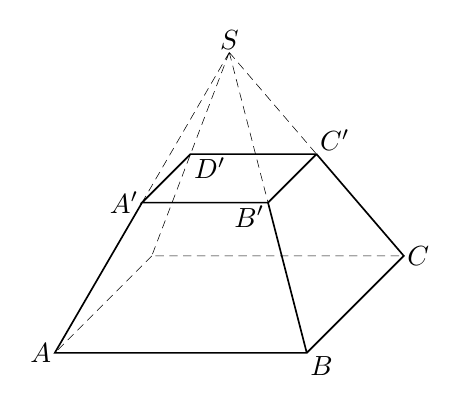
\begin{tikzpicture}[>=latex,scale=0.8,inner sep=1pt]
  \draw[semithick](-1,2,1)node[left]{$A'$}--(-2,0,2)node[left]{$A$}--(2,0,2)node[below right]{$B$}--(2,0,-2)node[right]{$C$}--(1,2,-1)node[above right]{$C'$}--(-1,2,-1)node[below right]{$D'$}--(-1,2,1)--(1,2,1)node[below left]{$B'$}--(1,2,-1)(2,0,2)--(1,2,1);
  \draw[very thin,densely dashed] (0,4,0)node[above]{$S$}--(-2,0,-2)--(2,0,-2)(-2,0,-2)--(-2,0,2)(0,4,0)--(1,2,1)(0,4,0)--(1,2,-1)(0,4,0)--(-1,2,1);
\end{tikzpicture}
\end{document}